\section{Iteration 5: Decomposition of the Scheduler for Anomaly Detection}
\label{add:it5}

\subsection{Step 1: Identify candidate drivers}
\label{add:it5/drivers}

\npar This iteration is driven by:

\begin{itemize}
	\item P1': Timely closure of valves. Alarm trames have to be handled within a bounded time. 
	\item P2': Anomaly Detection. When the system is in overload modus the processing order of trames
	  occurs on a priority basis (premium service has a higher priority than
	  normal service).
\end{itemize}

\npar No use cases were delegated to this component.

\subsection{Step 2: Choose design concepts}
\label{add:it5/concepts}

\npar The design concepts for this decomposition are completely analogous to the
design concepts of iteration 3 (see section \ref{add:it3/concepts}). 

\subsection{Step 3: Instantiate architectural elements and allocate responsibilities}
\label{add:it5/elements}

\npar Also analogous to iteration 3 (see \ref{add:it3}), an ADScheduler will
enqueue processing jobs with a priorities in an ADQueue with an ADPolicy. An
ADQueueReader will dequeue jobs from the queue en feed them
to the Anomaly Detection Unit. 

\npar An overview of the instantiated child components of the Anomaly Detection
Scheduler is shown in \ref{fig:it5/elements}.

\begin{figure}[H]
	\begin{centering}
		% TODO Figure
		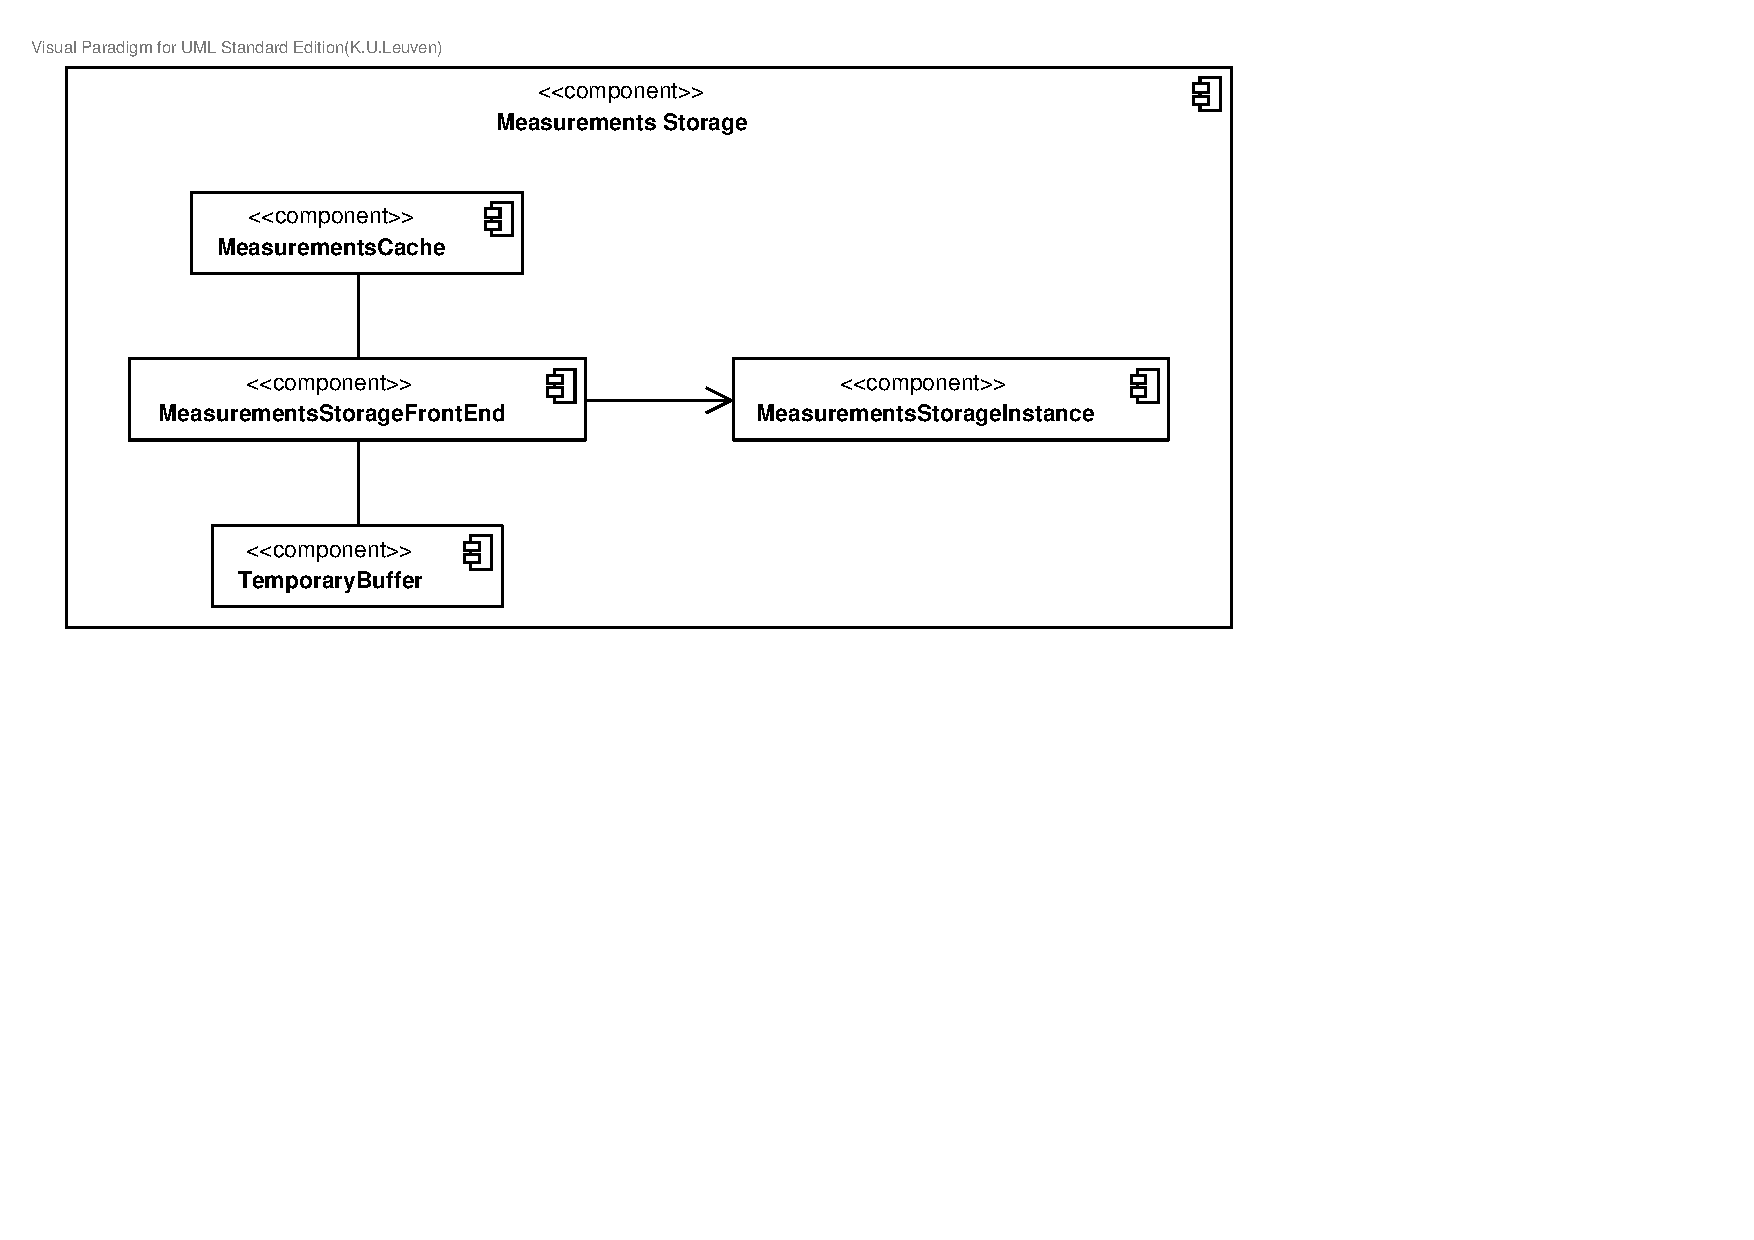
\includegraphics[width=\textwidth]{figs/add-it4-elements.pdf}
		\caption{Overview of all instantiated child elements in the Anomaly
		Detection Scheduler}
		\label{fig:it5/elements}
	\end{centering}
\end{figure}

\subsection{Step 4: Define interfaces for instantiated elements}
\label{add:it5/interfaces}

\npar Because this scheduler is very similar to the measurements scheduler from
iteration 3 (see \ref{add:it3}), the interfaces are also very similar. 

\npar Analogous to iteration 3, jobs are given in the form of ADCommands. An
ADCommand is an encapsulation of an anomaly detection request. This object
contains a copy of the received trame and the necessary data to fetch the
historical measurement data, the alarm data and the configuration data for this
device. This data will be used to determine whether an alarm is a false positive. 

\subsubsection{ADScheduler}

\npar The ADScheduler provides an interface
\interface{ADSchedulerAPI}. This interface contains a method
\method{shedule(ADCommand)} to schedule new commands.

\subsubsection{ADPolicy}

\npar The ADCommand will be placed in the ADQueue by a policy. Therefore,
ADPolicy provides an interface \interface{ADPolicyAPI} which contains a method
\method{insertCommand(ADCommand, ADQueue)}.

\subsubsection{ADQueue}

\npar The ADQueue must provide methods for inserting items and removing items.
These methods are contained in the \interface{ADQueueAPI} and are called
\method{insertCommand(ADCommand, double)} and \method{remove()}. The first
method is used by ADPolicy and the last one is used by ADQueueReader.

\npar Figure \ref{fig:it5/interfaces} summarizes the components and the
interfaces instantiated in this iteration.

\begin{figure}[H]
	\begin{centering}
		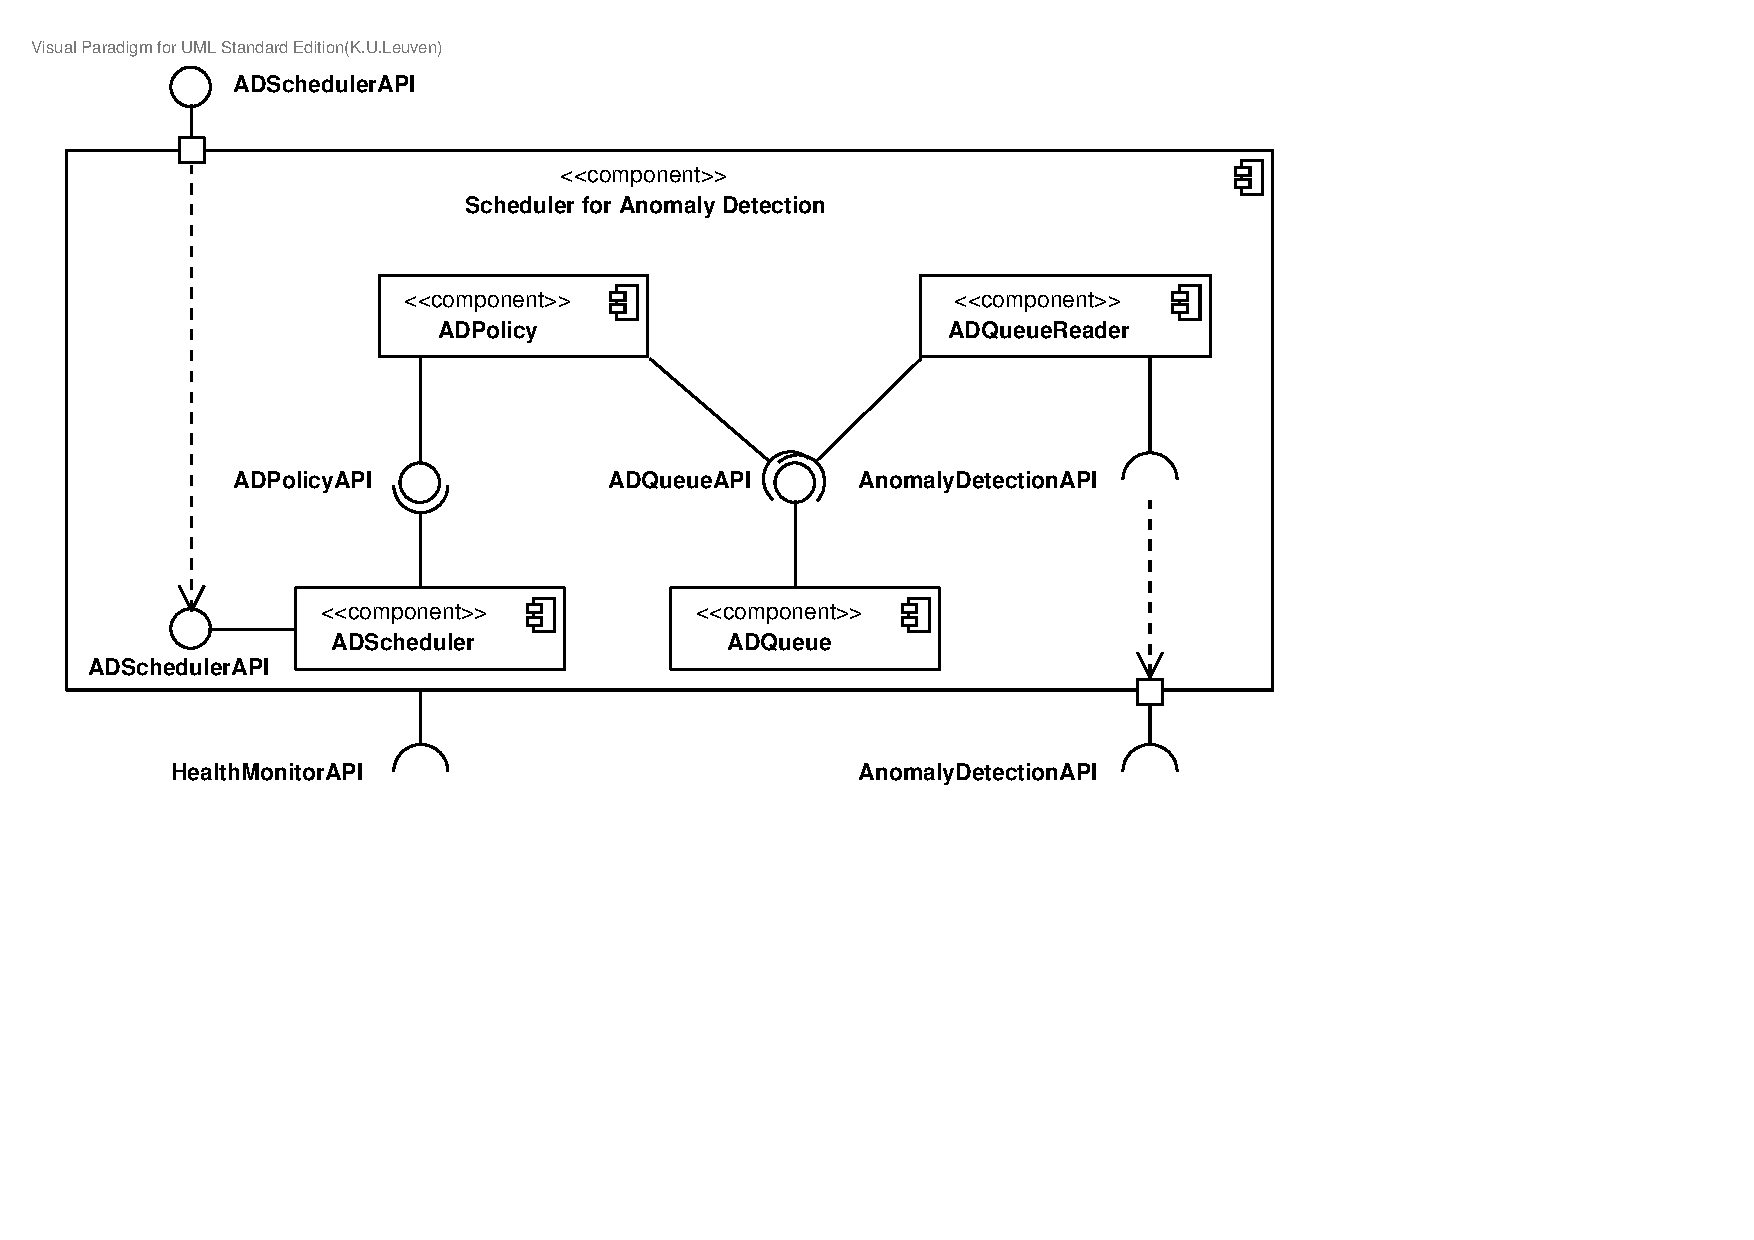
\includegraphics[width=\textwidth]{figs/add-it5-interfaces.pdf}
		\caption{Overview of the interfaces and components in the Anomaly Detection
		Scheduler}
		\label{fig:it5/interfaces}
	\end{centering}
\end{figure}

\subsection{Step 5: Verify and refine}
\label{add:it5/verification}

\npar All quality requirements are resolved in this iteration. The policies for
the scheduler will ensure that commands are scheduled in the right order. 
